\renewcommand{\theequation}{\theenumi}
\begin{enumerate}[label=\arabic*.,ref=\thesubsubsection.\theenumi]
\numberwithin{equation}{enumi}
\item  
$\vec{A}=\myvec{-1\\7}, \vec{B}=\myvec{4\\-3}$
\\
Then $\vec{C}$ that divides $\vec{A},\vec{B}$ in the ratio $k:1$ is
\begin{align}
\label{eq:3.6.1_section}
\vec{C}=\frac{k\vec{A}+\vec{B}}{k+1}
\end{align}
For the given problem k=$2:3$
\\
Using the equation \ref{eq:3.6.1_section}, the desired point is
\begin{align}
\vec{C}=\frac{\frac{2}{3}\myvec{-1\\7}+\myvec{4\\-3}}{\frac{2}{3}+1}
\\
\therefore \vec{C}=\myvec{2\\1}
\end{align}
The following code plots Fig.  \ref{fig:3.6.1_section}
\begin{lstlisting}
codes/line/section.py
\end{lstlisting}
\begin{figure}[!ht]
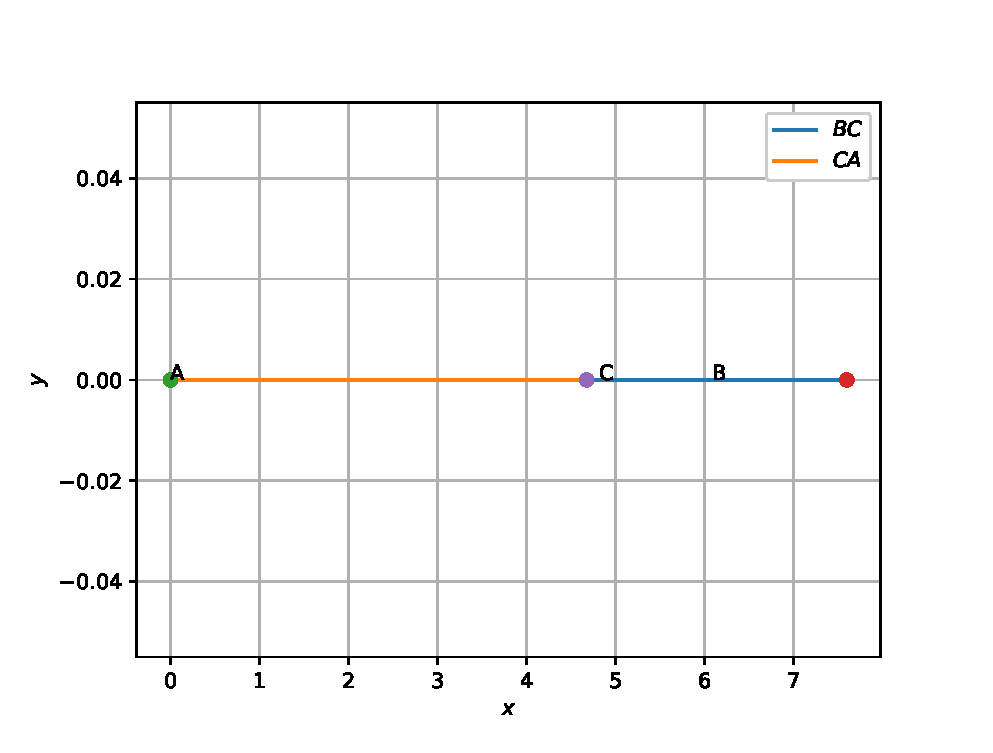
\includegraphics[width=\columnwidth]{./solutions/1/figs/line/section.eps}
\caption{}
\label{fig:3.6.1_section}
\end{figure}
\end{enumerate}
